% !TEX root = thesis.tex
\chapter{Evaluating the Need for CSS Code Conventions}
\label{sec:evaluating}

\section{Research Method}

Despite the new features added in the second~\cite{CSS2} and third~\cite{CSS3} versions of CSS, the
language has obvious limitations, for example, lack of variables. A number of preprocessors have
evolved to tackle the downsides of CSS. Solutions such as SASS~\cite{SASS}, LESS~\cite{LESS} and
Stylus~\cite{Stylus} offer enhanced or even different syntax and translate it to CSS. Preprocessors
are not only ubiquitously recommended, but also widely adopted in practice. The presence of such
solutions poses the question whether conventions for CSS are required at all. If nowadays CSS is
generated and not maintained, the need for CSS conventions is substituted with need for preprocessor conventions.

To determine whether CSS is still handcrafted, all commits to open source repositories hosted on
GitHub for the period Jan-Apr 2015 were analyzed. To differentiate between plain CSS and
preprocessor code, the extensions of all files in the commits were inspected. In case the commit
contains a file with extension \texttt{.scss}, \texttt{.sass}, \texttt{.less} or \texttt{.styl}, it
is considered preprocessor maintenance. In case the commit contains files with the \texttt{.css}
extension and no preprocessor extensions, it is considered maintenance of plain CSS. Since the main
objective of the search is finding maintained files, only files that have been modified are taken
into consideration. Files that have been added are excluded from the results, since developers often
add third-party CSS libraries to their repositories.


\section{Results}

A total of 1,589,713 commits to 1,311,654 public repositories have been analyzed. X of these were
not processed due to errors. Typical errors contain repositories that have been turned private
and... The number of commits that maintain any form of CSS is X. Figure \ref{cssresults} summarizes
the findings.

\begin{figure}[h!]
  \centering
  \caption{Results}
  \label{cssresults}
  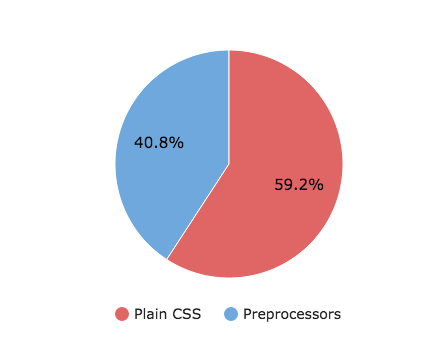
\includegraphics[width=0.5\textwidth]{cssresults}
\end{figure}

\section{Analysis}

There are a number of limitations that need to be considered before interpreting the results of the
conducted research. Firstly, the search is conducted on a single hosting platform - GitHub. That
said, currently GitHub reports having over 10 million users and 24 million
repositories~\cite{GitHub}, which makes it the largest code host in the
world~\cite{gousios2014lean}. Secondly, the search is narrowed to the publicly available
repositories. Thus, it lies on the premise that there is not a significant difference between the
public and private repositories hosted on the platform. Thirdly, the search detects only the four
most popular preprocessor extensions and omits other preprocessors. It is possible that a number of
custom preprocessors are used in practice. However, it is assumed that the number of such commits
would not increase the number of total CSS commits to the extend at which the percentage of plain
CSS commits is significantly diminished.

Having the above limitations in mind, the search provides evidence to conclude that despite the
popularity of preprocessors, plain CSS is still handcrafted on GitHub in the beginning of 2015.

